\documentclass{beamer}

\title{Modelos Generativos Profundos}
\subtitle{Clase 3: Introducción a las redes bayesianas}
\author{Fernando Fêtis Riquelme}
\institute{
    Facultad de Ciencias Físicas y Matemáticas\\
    Universidad de Chile
}
\date{Otoño, 2025}
\titlegraphic{\hfill
\includegraphics[height=1.2cm]{fcfm}}

\usetheme{metropolis}
\setbeamercovered{transparent}

\begin{document}

\begin{frame}
    \titlepage
\end{frame}

\begin{frame}{Clase de hoy}
    \tableofcontents
\end{frame}

\section{Ejemplo inicial}

\begin{frame}{Ejemplo de red bayesiana}
    Se definirán 4 variables aleatorias binarias asociadas a un modelo probabilístico de juguete.
    \begin{itemize}
        \item<2-> \textbf{Variable aleatoria $x_1$:} el estudiante estudia para el examen.
        \item<3-> \textbf{Variable aleatoria $x_2$:} el estudiante responde bien las preguntas teóricas.
        \item<4-> \textbf{Variable aleatoria $x_3$:} el estudiante responde bien las preguntas prácticas.
        \item<5-> \textbf{Variable aleatoria $x_4$:} el estudiante aprueba el curso.
    \end{itemize}
    \uncover<6>{El valor $1$ estará asociado a la respuesta \texttt{sí} mientras que el valor $0$ estará asociado a la respuesta \texttt{no}.}

\end{frame}

\begin{frame}{Relaciones de dependencia del modelo}
    \begin{columns}

        \begin{column}{0.6\textwidth}
            \vspace{1.5cm}\\
            Se considerarán las siguientes relaciones de dependencia directa entre las 4 variables:
            \begin{equation*}
                p(x_1,x_2,x_3,x_4) = p(x_1)p(x_2|x_1)p(x_3|x_1)p(x_4|x_2,x_3)
            \end{equation*}
        \end{column}
        \begin{column}{0.39\textwidth}
            \centering\vspace{1cm}
            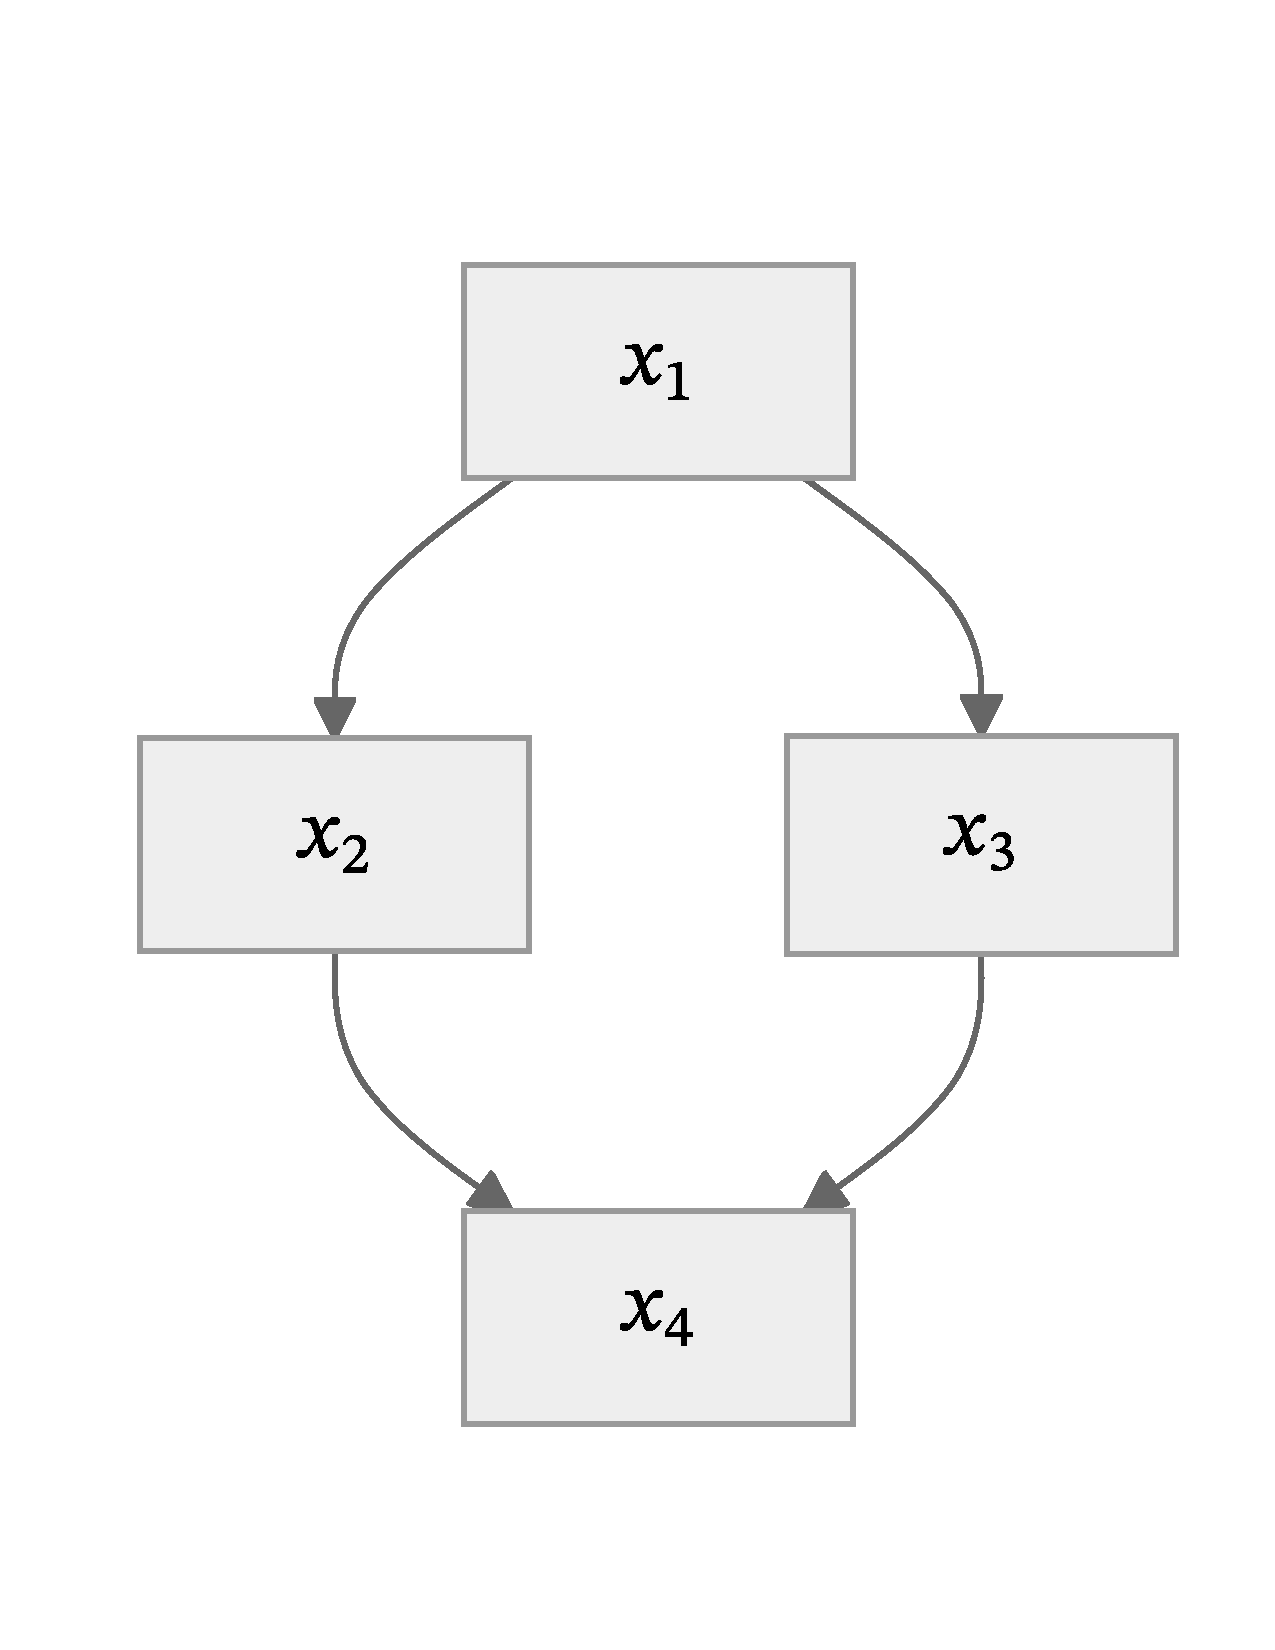
\includegraphics[width=\columnwidth]{net}
        \end{column}
    \end{columns}
\end{frame}

\begin{frame}{Distribuciones condicionales}

    El modelo $p(x_1,x_2,x_3,x_4) = p(x_1)p(x_2|x_1)p(x_3|x_1)p(x_4|x_2,x_3)$ necesita definir 4 distribuciones.
    \vspace{-0.5cm}
    \begin{columns}
        \begin{column}{0.45\textwidth}
            \centering
            % p(x1):
            \uncover<2>{
                \begin{table}
                    \centering
                    \resizebox{\columnwidth}{!}{
                        \begin{tabular}{|c|c|}
                            \hline
                            $p(x_1=0)$ & $p(x_1=1)$ \\ \hline
                            $0.10$     & $0.90$     \\ \hline
                        \end{tabular}
                    }
                \end{table}
            }
            % p(x2|x1):
            \uncover<3>{
                \begin{table}
                    \centering
                    \resizebox{\columnwidth}{!}{
                        \begin{tabular}{|c|c|c|}
                            \hline
                            $x_1$ & $p(x_2=0|x_1)$ & $p(x_2=1|x_1)$ \\ \hline
                            $0$   & $0.80$         & $0.20$         \\ \hline
                            $1$   & $0.25$         & $0.75$         \\ \hline
                        \end{tabular}
                    }
                \end{table}
            }
            % p(x3|x1):
            \uncover<4>{
                \begin{table}
                    \centering
                    \resizebox{\columnwidth}{!}{
                        \begin{tabular}{|c|c|c|}
                            \hline
                            $x_1$ & $p(x_3=0|x_1)$ & $p(x_3=1|x_1)$ \\ \hline
                            $0$   & $0.70$         & $0.30$         \\ \hline
                            $1$   & $0.20$         & $0.80$         \\ \hline
                        \end{tabular}
                    }
                \end{table}
            }
        \end{column}
        \begin{column}{0.55\textwidth}
            \centering
            \uncover<5>{
                \begin{table}
                    \centering
                    \resizebox{\columnwidth}{!}{
                        \begin{tabular}{|c|c|c|c|}
                            \hline
                            $x_2$ & $x_3$ & $p(x_4=0|x_2,x_3)$ & $p(x_4=1|x_2,x_3)$ \\ \hline
                            $0$   & $0$   & $0.95$             & $0.05$             \\ \hline
                            $1$   & $0$   & $0.35$             & $0.65$             \\ \hline
                            $0$   & $1$   & $0.40$             & $0.60$             \\ \hline
                            $1$   & $1$   & $0.01$             & $0.99$             \\ \hline
                        \end{tabular}
                    }
                \end{table}
            }
        \end{column}
    \end{columns}
\end{frame}

\begin{frame}{Preguntas}
    Conocer las distribuciones del modelo probabilístico permite responder preguntas acerca de las variables aleatorias involucradas.
    \begin{itemize}
        \item<2> ¿Cuál es la probabilidad de que el estudiante responda bien las preguntas teóricas?
        \item<3> ¿Cuál es la probabilidad de que el estudiante haya estudiado si no respondió bien las preguntas teóricas?
        \item<4> ¿Cuál es la probabilidad de responder bien tanto las preguntas teóricas como las preguntas prácticas?
        \item<5> ¿Cuál es la probabilidad de responder bien las preguntas prácticas si se respondieron bien las preguntas teóricas?
    \end{itemize}
\end{frame}

\section{Formulación de una red bayesiana}

\begin{frame}{Aprendizaje de una distribución conjunta}
    Se busca modelar una distribución conjunta $p(x_1,\ldots,x_N)$. Por qué no usar KDE?
    \begin{itemize}
        \item<2>Distribución empírica.
        \item<3>Kernel density estimation.
    \end{itemize}
\end{frame}

\begin{frame}{Modelos gráficos generativos}
    Una red bayesiana utiliza un grafo dirigido acíclico para representar la distribución conjunta de un modelo probabilístico.
    \begin{itemize}
        \item<2> \textbf{Algunos conceptos de grafos:} camino dirigido, DAG, nodos padres, orden topológico.
        \item<3> \textbf{Factorización de una red bayesiana:} propiedad de Markov.
        \item<4> \textbf{Modelos de variable latente:} reducción de dimensionalidad, interpolación en el espacio latente, manipulación de atributos.
    \end{itemize}
\end{frame}

\begin{frame}{Algunas redes bayesianas}
    \begin{itemize}
        \item<2> \textbf{Modelos clásicos en ML:} naïve Bayes, mixturas, cadenas de Markov, HHMs.
        \item<3> \textbf{Modelos generativos modernos:} ARMs, VAEs, GANs, DMs, NFs.
        \item<4> \textbf{Modelos generativos condicionales:} modalidades, arquitectura, comparación con modelos discriminativos.
        \item<5> \textbf{Generación de nuevas muestras:} ancestral sampling, MCMC.
    \end{itemize}
\end{frame}

\begin{frame}{Inferencia}
    \begin{itemize}
        \item<1> Por lo general, las distintas redes bayesianas están motivadas por ideas simples.
        \item<2> Lo que es más difícil es lograr obtener los parámetros de las distribuciones involucradas. Cada paradigma utiliza un enfoque distinto.
        \item<3> Esto es necesario para que el modelo sea similar a la distribución que busca modelar.
    \end{itemize}
\end{frame}

\begin{frame}{Próxima clase}
    En la próxima clase.
    \begin{itemize}
        \item<2> Se estudiará el problema de inferencia en redes bayesianas.
        \item<3> Se revisará el enfoque de máxima verosimilitud junto a sus limitaciones.
    \end{itemize}
\end{frame}

\begin{frame}
    \centering
    \Large{Modelos Generativos Profundos}\\
    \large{Clase 3: Introducción a las redes bayesianas}
\end{frame}

\end{document}